\documentclass{beamer}

\usecolortheme{seahorse}
\setbeamertemplate{navigation symbols}{}

\usepackage{pdfpages}

\usepackage{polyglossia}
\setmainlanguage{russian}
\setmainfont{Liberation Serif}
\setsansfont{Liberation Sans}

\title{Системный язык программирования с зависимыми типами}
\author{Соколов Павел}
\date{24 января 2024}

\begin{document}

\frame{\titlepage}

\begin{frame}{Путь к линейным зависимым типам}
  \begin{itemize}
    \item Categorical Semantics of Linear Logic (2009) --- исследование
      категорной семантики линейной логики
    \item Syntax and Semantics of Linear Dependent Types (2014) --- нет
      зависимости от линейных типов
    \item I Got Plenty o’ Nuttin’ (2016) и другие QTT
    \item A Bunched Homotopy Type Theory for Synthetic Stable Homotopy Theory
      (2022) --- зависимость через ``marked'' вхождения в тип, аналог
      модальности $!$ в линейной логике
  \end{itemize}
\end{frame}

\includepdf[pages={6-20}]{Riley-2022-01-20-HoTTEST.pdf}

\begin{frame}{Типы указателей, типы допуска}
  Аналогично ATS и GhostCell (2021), за адресацию и за владение памятью
  отвечают два разных типа: тип ссылок $\& A$ и, для любых $r : \& A$ и
  $n : \mathrm{nat}$, допуск $[r; n)$.

  Некоторые свойства:
  \begin{itemize}
    \item $\& A$ не является линейным;
    \item над $\& A$ можно производить арифметику на указателях;
    \item $[r; n)$ является линейным;
    \item $\textcolor{blue}{\boldsymbol{[}}r; n\textcolor{blue}{\boldsymbol{)}}$
      можно разделять (на $\textcolor{blue}{\boldsymbol{[}}r; m)$ и
      $[r + m; n\textcolor{blue}{\boldsymbol{)}}$) и соединять обратно;
    \item Чтение и запись по $p : \& A$ можно производить только при наличии
      $[r; n)$ такого, что $r : \& A$ и $r \leq p < r + n$.
  \end{itemize}
\end{frame}

\begin{frame}{Ручное управление памятью}
  На основе типов данных, введённых ранее, можно ввести следующие операции:

  \[
    \mathrm{malloc}_A : (n : \mathrm{nat}) \multimap \mathrm{ENOMEM}
      \oplus (r : \& A) \otimes
      \textcolor{blue}{\boldsymbol{[}}r; n\textcolor{blue}{\boldsymbol{)}}
  \]

  \[
    \mathrm{realloc}_{A, r, n} : (m : \mathrm{nat}) \otimes
      \textcolor{blue}{\boldsymbol{[}}r; n\textcolor{blue}{\boldsymbol{)}}
      \multimap
      \textcolor{blue}{\boldsymbol{[}}r; n\textcolor{blue}{\boldsymbol{)}}
      \oplus
      (r' : \& A) \otimes
      \textcolor{blue}{\boldsymbol{[}}r'; m\textcolor{blue}{\boldsymbol{)}}
  \]

  \[
    \mathrm{free}_{A, r, n} :
      \textcolor{blue}{\boldsymbol{[}}r; n\textcolor{blue}{\boldsymbol{)}}
      \multimap 1
  \]

  Благодаря выразительности базовой системы типов соотношения, которым должна
  удовлетворять модель такой сигнатуры, можно выписать внутри теории. Возможные
  вариации операционных моделей с состоянием очевидны.
\end{frame}

\begin{frame}[fragile]{Задача 1: эффективная компиляция лямбда-выражений}
  \begin{enumerate}
    \item Стандартное решение в C++, Rust: анонимный тип данных, сохраняющий
      контекст, с переопределённой операцией \verb|()|.
      \begin{itemize}
        \item Недостаток: нет одного типа функции $(x : A) \to B(x)$, есть
          семейство типов, объединённых одним концептом (C++) / трейтом (Rust).
      \end{itemize}
    \item Есть boxed вариант, в котором контекст хранится в куче, так что
      ``лямбда'' представляется в виде пары указателей --- на данные и на
      функцию. Недостатки:
      \begin{itemize}
        \item Потеря производительности по сравнению с первым вариантом;
        \item Решение полагается на работу с кучей.
      \end{itemize}
    \item Заметим, что куча нужна только для того, чтобы обойти проблему с
      контекстами разной длины. Для решения на стеке можно дополнительно хранить
      в структуре её размер.
  \end{enumerate}
\end{frame}

\begin{frame}{Задача 2: (ко-)рекурсивные типы данных (I)}
  \begin{itemize}
    \item Аналогично задаче с лямбдами, представление индуктивных типов
      данных в памяти вынуждено использовать кучу; здесь обойти это ограничение
      не представляется возможным.
    \item Кроме этого, в системном программировании повсеместно используются не
      завершающиеся процедуры и явно циклические типы данных (например,
      двусвязный список). Для их моделирования в языках с зависимыми типами
      используются ко-данные и ко-рекурсия.
  \end{itemize}
\end{frame}

\begin{frame}{Задача 2: (ко-)рекурсивные типы данных (II)}
  \begin{itemize}
    \item Для аккуратного анализа работы с ко-данными используется guarded
      recursion, см. Productive Coprogramming with Guarded Recursion (2013).
    \item Предложение: для представления ко-данных использовать типы вида
      $\nu A. F(\& A)$, для индуктивных типов данных ---
      $\mu A. F((r : \mathrm{nat}) \otimes [r; 1))$.
    \item Индуктивные линейные типы --- тема новейших исследований, см.
      A Calculus of Inductive Linear Constructions (2023).
    \item Направление дальнейших исследований --- интеграция системы из статьи
      выше в нашу, исследование эргономики и её повышение.
  \end{itemize}
\end{frame}

\end{document}
